\section{Analysis of Categorical Data}

\subsection{Graphical Descriptive Methods}
\begin{objectives}
\item Briefly review the graphs for presenting categorical data
\item Know the advantages of various graphs
\end{objectives}
\vbox{}
After doing the research and getting a bunch of categorical Raw Data, it's important for us to sort and represent this data in a clear and efficient way so that we can do the following analysis of data.\\
\begin{Center}
    \Index{Comparative Bar Chart}
\end{Center}
This kind of bar charts can give a straightforward comparison between different groups in terms of the \textbf{Relative Frequency}. But remember when comparing, we compare the \textbf{Relative Frequency} instead of frequency.
\begin{figure}[H]
            \centering
            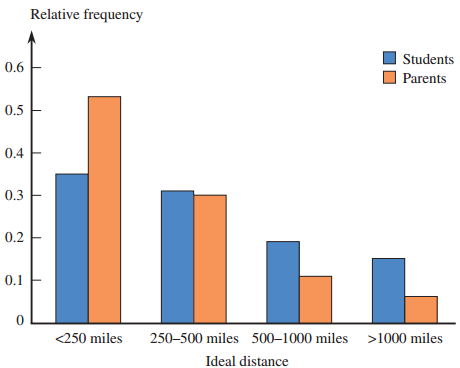
\includegraphics[width=75mm]{cbc.png}
            \caption{Comparative Bar Chart}
            \label{Comparative Bar Chart}
        \end{figure}
\begin{Center}
    \Index{Pie Chart}
\end{Center}
The proportion of each category is representing by the size of its correlated segment's area. So it is straightforward to see the \textbf{Relative Frequency} of each category.
        \begin{figure}[H]
            \centering
            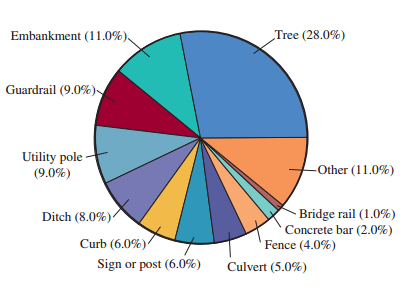
\includegraphics[width=75mm]{pie_chart.png}
            \caption{Pie Chart}
            \label{pie chart}
        \end{figure}
\begin{Center}
    \Index{Segmented Bar Chart}
\end{Center}
It is almost the same as Pie Chart. Instead of a circle , the Segmented Bar chart is a rectangular. It is also straightforward to see the \textbf{Relative Frequency} of each category.
    \begin{figure}[H]
            \centering
            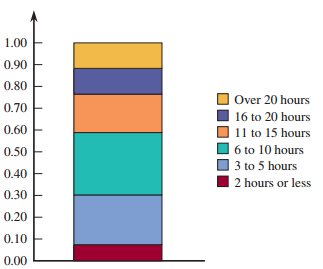
\includegraphics[width=75mm]{segmented_bar_chart.png}
            \caption{Segmented Bar Chart}
            \label{segmented bar chart}
        \end{figure}

\subsection{Numerical Descriptive Methods}
\begin{objectives}
    \item Understand Frequency, Relative Frequency and Proportion of Success
    \item Know how to calculate Relative Frequency and Proportion of Success
\end{objectives}
\vbox{}
Besides representing data by using graphs, there are also two most important features of each category in a research: \textcolor{red}{Frequency} and \textcolor{red}{Relative Frequency}, also there is a special type of Relative Frequency is called \textcolor{red}{Proportion of Success}.\\
\begin{description}
    \item \Index{Frequency}: Frequency is the number of times the category appears in the data set. 
    \item \Index{Relative Frequency}:Relative frequency is the proportion of a certain category within all data.
    \begin{examplebox}{Frequency and Relative Frequency}
    We conduct an interview about BNDS students' favorite color. And there are 500 results in total. Among all these results, the color "red" appears for 50 times, so its frequency is 50, relative frequency is 50/500=0.1.
    \end{examplebox}
    \item \Index{Proportion of Success}: A special relative frequency, when the data has only two categories, we can define one as success and the other one as failure.\\
    \begin{examplebox}{Proportion of Success}
        We are testing BNDS students' AP statistics scores. A 5 is success, a below 5 is failure. And among 100 students, 95 get a 5. So the proportion of success is 95/100=0.95.
    \end{examplebox}
\end{description}

\subsection{Proportion of Success}
\begin{objectives}
    \item Understand dychotomy and proportion of success
    \item Know how do infer Confidence Level of \(\Pi\)
    \item Know how to do hypothesis test of \(\Pi\)
    \item Understand difference of proportion of success
    \item Know how to do confidence interval and hypothesis test for difference of proportion of success
\end{objectives}
\vbox{}
For categorical data, there is a very special case, which has only two categories.\\

\begin{description}
    \item \Index{Dychotomy} : When there are only two possible cases in uni variate data, and we can assign each case as either \textcolor{blue}{success} and \textcolor{blue}{failures}.
    \item \Index{Binomial Distribution} : Used to analyze Dychotomy and as long as n is greater than 30, and the skewness is not too extreme  the Binomial Distribution can be approximate by a \textcolor{red}{Normal Distribution} with the same Mean and Standard Deviation.
    \item \Index{Proportion of Success} : In the Binomial Distribution
    \begin{equation}
        \Pi=\frac{x}{n}
    \end{equation}
    \textbf{x} is number of success in \textbf{n} trials.
    \item \Index{Probability of Success on a trial} : it's denoted by \textbf{p}, it's the same as \(\Pi\). Also, the \(1-p\) is \textbf{q}.
        \begin{equation}
        p=\frac{x}{n}
    \end{equation}
\end{description}

Through a series of deduction, we attain the following equations for the \Index{Expected value of x} and \Index{Variance of x}.
\begin{equation}
    E(x)=np
\end{equation}
\begin{equation}
    Var(x)=np(1-p)
\end{equation}

If we have a sampling distribution for \(Pi\), the \textcolor{blue}{mean} and \textcolor{blue}{standard deviation} are as following:
\begin{equation}
    E(\Pi)=p    
\end{equation}
\begin{equation}
    Var(\Pi)=\frac{p(1-p)}{n}
\end{equation}

\vspace{5ex}
\begin{Center}
    \textbf{Confidence Interval of Proportion of Success}
\end{Center}
Using the equations above of mean and standard deviation, based on our study for Confidence Interval, we can attain the equation for \textcolor{red}{Confidence Interval of Proportion of Success}
\begin{equation}
    \Pi\in(\hat{p}\pm B_{C.L.}\sqrt{\frac{p(1-p)}{n}})
\end{equation}
As mentioned before: as long as n is greater than 30, and the skewness is not too extreme  the Binomial Distribution can be approximate by a \textcolor{red}{Normal Distribution} with the same Mean and Standard Deviation. \textcolor{blue}{\(B_{C.L.}\)} can be approximated by \textcolor{blue}{\(Z_{C.L.}\)}.\\
As for \textcolor{red}{\(\hat{p}\)}, it is the \textcolor{blue}{expected value of p}, which can be calculated by doing \(\frac{x}{n}\) of the sample.

\vspace{5ex}
\begin{Center}
    \textbf{Hypothesis Test of Proportion of Success}
\end{Center}
Based on the equations above and the test value we learnt before, we can attain the equation for the \textcolor{red}{Test Value}.
\begin{equation}
    Z_{T}=\frac{\hat{p}-\Pi_{0}}{\sqrt{\frac{\hat{p}(1-\hat{p})}{n}}}
\end{equation}
As for the test part, it's the same as before.

\vspace{5ex}
\begin{Center}
    \textbf{Sample Size of Proportion of Success}
\end{Center}
When we wish to design a dycholomous experiment, with certain \textcolor{blue}{Confidence Level} and \textcolor{blue}{Margin of Error}. The minimum required \textcolor{red}{Sample Size}:
\begin{equation}
    n=(\frac{Z}{M.E.})^2p(1-p)
\end{equation}
Without the information about the value of p, we take the max value of \(p(1-p)\) which is \(\frac{1}{4}\). Then the equation becomes:
\begin{equation}
    n=(\frac{Z}{2M.E.})^2
\end{equation}

\vspace{5ex}
\begin{paragraph}{Difference of Proportion of Success}
    When we are analyzing, sometimes we care more for the Difference of Proportion of Success between two population, first we discuss for \textcolor{red}{Independent Samples} . \\
    \begin{examplebox}{Difference of Proportion of Success}
           We want to know if the effect of drug changes the percentage of students with 5 on AP test, we concern more for if there is actually a difference for their proportion of success instead of the value of it.
    \end{examplebox}
 \end{paragraph}
 \vspace{6ex}
 \begin{Center}
     \textbf{Confidence Interval for Difference of Proportion of Success}
 \end{Center}
 For the confidence interval of difference of proportion of success, it's technically the same as for difference of mean. We change the expected value to the difference of proportion of success, and the standard deviation to the sum of two standard deviation.
 \begin{equation}
     (\Pi_1-\Pi_2)\in((\hat{p}_1-\hat{p}_2)\pm Z_{C.L.}\sqrt{\frac{\hat{p}_1(1-\hat{p}_1)}{n_1}+\frac{\hat{p}_2(1-\hat{p}_2)}{n_2}})
 \end{equation}
\(\hat{p}\) is just calculated from the sample's x and n, \(Z_{C.L.}\) approximates \(B_{C.L.}\).
\vspace{5ex}
\begin{Center}
    \textbf{Hypothesis Test for Difference of Proportion of Success}
\end{Center}
For the \textcolor{blue}{independent samples the difference of proportion test} is 
\begin{equation}
    Z_{T}=\frac{(\hat{p}_1-\hat{p}_2)-\Pi_0}{\sqrt{\frac{\hat{p}_1(1-\hat{p}_1)}{n_1}+\frac{\hat{p}_2(1-\hat{p}_2)}{n_2}}}
\end{equation}
Where \(\Pi_0=\Pi_1-\Pi_2\) is the hypothesized difference of proportions. And this only works for large n(more than 30).\\
\vspace{5ex}

If this is \textcolor{red}{dependent samples}, then the variance of the difference of proportions should not simply be the sum of two variances, it is:
\begin{equation}
    Var(\hat{p}_1-\hat{p}_2)=Var(\hat{p}_1)+Var(\hat{p}_2)-2Covar(\hat{p}_1,\hat{p}_2)
\end{equation}
Whern \(Covar(\hat{p}_1,\hat{p}_2)\) is resulted by the relation of two samples, and it is:
\begin{equation}
    Covar(\hat{p}_1,\hat{p}_2)=-\frac{\hat{p}_1\hat{p}_2}{n}
\end{equation}
Here, we are assuming that \textcolor{blue}{sample size of two populations are the same n}. \\
Except for the variation of variance, the other processes are exactly the same with independent samples.